\refstepcounter{tdel}
\section{Technical Deliverable \thetdel\ -- Does E4L allow for easy
deployment of adjacent Microservices?}
\label{td:ms}

\subsection{Requirements}

Our case study consisted in creating a \gls{ms} relying on the
\gls{e4l} application. The latter is built using a monolithic
architecture, and we want to find out how easy it is to deploy an
adjacent \gls{ms} application.

The \gls{ms} to be created should allow us to test the hypothesis that
\glspl{ms} are easy to create and deploy. Further, it should fit into
our \gls{e4l} case study---we will have our service display a graph
based on data collected by the \gls{e4l} application; figure
\vref{fig:dash-api} shows an example of our graph.  To close
everything off, we shall also create a GitLab pipeline that automates
the deployment of this \gls{ms}.

\begin{figure*}
	\centering
	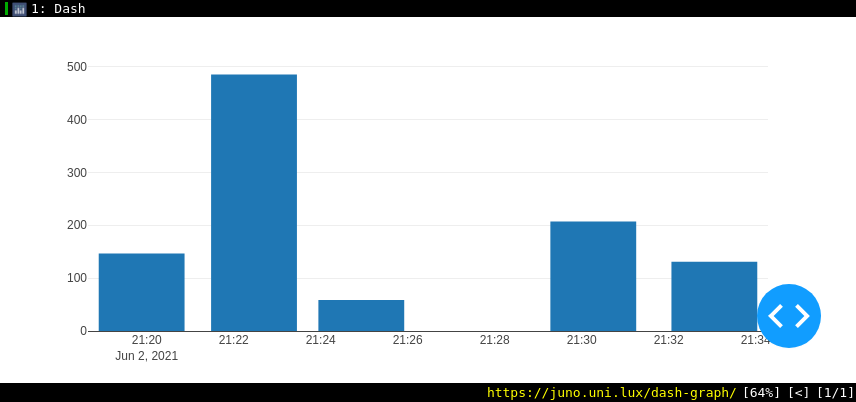
\includegraphics[width=\linewidth]{images/dash-API-demo.png}
	\caption{\gls{ms} graph relying on \gls{e4l} API}
	\label{fig:dash-api}
\end{figure*}

Hence, the design section will tackle all the steps we had to
undertake in order to reach the final and fully automated deployment
pipeline. The production section will dive into the technical details
and difficulties of each step. The assessment is going to lay out our
judgement on how easy it was to deploy the \gls{ms} given the current
\gls{e4l} application architecture.

\subsection{Design}

\subsubsection{Set up repository}

The first step was to set up a repository in which we could place our
productions. I had to request an account in order to access the
\url{https://gitlab.uni.lu} GitLab service. An interesting thing to
note at this point being that this GitLab service will host our
\gls{ms} code on a different server from the one that contains the
\gls{e4l} code. Thus we can further verify the independence of such
services.

\subsubsection{Familiarize with docker}

We then had to get familiar with the \textit{docker} utility and how
to create and manage containers with it. This tool is what would
effectively allow us to create isolated services by containerising our
application into a docker container.

The rationale behind using docker instead of simply running a process
directly comes back to the points mentioned in the
\nameref{sec:componentization} section. Simple processes would not
enforce the \gls{ms} architecture as much as containers would, thus
allowing for development to shift into a monolithic architecture.

At a later stage we also inspected the \textit{docker-compose}
utility which allows for finer and more automated management of
containers.

It is also interesting to note at this point that evidence suggests
docker to be quite difficult to use and get started with for the
average developer. Many times you would find Stack Overflow posts
asking about very basic concepts over a broad range of disciplines and
even the docker utility in itself. \cite{docker-so} Given that docker
indeed encompasses a broad range of disciplines, it may take some time
for specialists in one field to adapt to this new paradigm.

\subsubsection{Familiarize with CI/CD}

In order to automate the deployment of our application, we want to
take advantage of GitLab's \gls{cicd} framework. At this point in time
our \gls{ms} was not fully functioning yet and we were simply
experimenting with dummy code. The main goal here was to understand
how it works and what it does.

Creating the actual pipeline for our finished \gls{ms} was only the
very last step of the process. The rationale is that automating such a
procedure can only be done if one is familiar with the steps that
would otherwise need to be done manually. Therefore it was important
to work out everything by hand before finalizing with an automated
pipeline.

\subsubsection{Obtain data from E4L}

Since our \gls{ms} would display a graph using data from \gls{e4l}
responses, we had to find out how to extract this information. Finding
this out was quite an extensive process in itself since the hints were
not too clearly laid out in the documentations. More details will be
provided in the production.

To give an outline, our first attempt was to sort of brute-force our
way into obtaining data. While not the most useful of data, it was
something to work with. Only later have we discovered that \gls{e4l}
exposes an API which greatly alleviates the burden of our brute-force
approach.

Obtaining useful data however, was only achievable thanks to the help
and guidance of a prior team member of \gls{e4l} who had great
responsibility in creating the back-end. He showed me the proper way to
obtain all the data from the API as well as by directly connecting to
the \gls{e4l} database.

\subsubsection{Write code which retrieves data and displays it}

For this purpose we relied on productions made during my summer job
where I was responsible for finding ways to plot graphs. For the sake
of simplicity we used Python to write this code. It should be noted
that this and the previous step of obtaining data were always running
in parallel.

In the end, it was simply a matter of retrieving the data from the API
or the database, and then to plot some data using example code
produced during the summer job. It should further be noted that we
were not deeply interested in \textit{what} data is being displayed, it should
rather serve as a proof of concept for our purpose.

\subsubsection{Containerize the application}

Once the application was working locally, we attempted to make it run
inside a docker container. Note that only the version retrieving data
from the API was used for experimenting this way. The database version
is analogous and did not require great modifications. Further it had a
restriction where the database was only accessible to certain docker
containers running on the server where the database lives. We will
provide more details in the production.

Containerizing the application came with a fair share of issues
however both locally as well as once deployed on the testing server.
Work-arounds and fixes were implemented an resulted in a fully
functional service.

\subsubsection{Create pipeline to automate deployment}

The final step was to create a pipeline that automates the whole
process of deploying the application to Juno. Since we were making a
Python application, there were no building stages that had to be made
in the pipeline. Thus we only ended up with a deployment stage which
was very short thanks to the docker-compose utility taking care of
everything.

\KB{Methodlogy: Steps required to achieve final solution}

\subsection{Production}

% \KB{More details on each step + difficulties encountered}

\KB{screenshot showing final product: E4L page with graph}

\KB{Reference \textit{replication package} in README of
code/repository}


\subsubsection{Set up repository}

Once access to GitLab was obtained, it was relatively straight forward
to create a new repository. The only special thing we did was to host
the repository under a group instead of the personal space. This would
later allow us to have shared GitLab runners for executing the
pipelines.

Projecting a little, nothing would have prevented us from setting up
project specific runners for our two solutions, but given they require
the same type of runner it made sense to share a runner, thus the
rationale for creating the projects under a group.

\subsubsection{Familiarize with docker}

Besides following tutorials, we also played around with the tool in
order to better grasp how it works. For example we wrote a simple
hello world program in C. We then tried compiling it before building
the container and only put the binary into it. And we tried compiling
the program while building the container.

\subsubsection{Familiarize with CI/CD}

Better understanding the \gls{cicd} pipeline was done in the same
fashion as for docker, using a bunch of experiments to understand how
it works. For instance again compiling the C program using docker, or
compiling it using the \gls{cicd} pipeline.

\subsubsection{Obtain data from E4L}

Our \gls{ms} should obtain data from \gls{e4l} and plot it using
a Dash/Plotly application. Obtaining the data was quite a journey
however, let us explore this process.

\paragraph{First attempt at obtaining data from the back-end}

Upon inspection of the \gls{e4l} backend, we were able to find a
potentially relevant endpoint that would allow us to query answers
from the questionnaire.  However, it quickly became apparent that the
back-end endpoints were specifically made to be used by the front-end
page. Further evidence for this can be found in the functionalities
described in the README, which also informs us that the only data that
can be extracted is specific to a session. All of this essentially
means that we have no direct way to access any data beyond what we are
presented with on the web page---which would only comprise our results
from after answering the questionnaire.

Upon completing the questionnaire in E4L, we are presented the
following page\footnote{Note that the ID will be different. This is an
example for a results page that we obtained at some point.}:
\url{https://juno.uni.lux/e4l/result/MzA5.-7-sMYXmv3tXyuLQT2s1ZgULRKY}.
The so-called	\textit{sessionId} is unique to our provided answers, so
by taking note of it we are able to review our \textit{energy scores}
at any point in time. The obvious course of action now would be to use
the \verb|/calculate/session/{sessionId}| endpoint---which is our only
of two GET handlers regarding the questionnaire---to obtain our
results.

\paragraph{Scraping the results page for data}

One problem rose quickly however: We had no information on where or
how to access the back-end in order to issue our GET request. Upon
inspection in the code for both the front-end and back-end, we were
unable to find any concrete traces on how to reach it. The closest we
managed to find was the definition of a \verb|baseUrl| using \verb|axios|,
but that still left us clueless. So we set out to create a web scraper
that would parse the HTML of the above results page.

We used \verb|selenium| to perform this task. However, running the
selenium browser in headless mode---as is required for running this
code in a docker container---caused issues with our scraper. It turns
out that the page contents would not be loaded unless the page was
actually rendered by the browser. In addition to this approach being
extremely slow due to \verb|selenium|, it was simply not usable for
our use-case.

\paragraph{Obtaining data from the back-end API}

It was only after a third and final inspection of the E4L
code---performed while documenting here what we did---with the help of
GitLab's search utility, that we discovered how to access the
back-end.  It was hidden in plain site in the front-end README,
however it was not emphasised very well which caused us to completely
overlook it at multiple occasions.

That said, we were able to retrieve our results using the API by
issuing a GET request on
\url{https://juno.uni.lux/e4lapi/calculate/session/MzA5.-7-sMYXmv3tXyuLQT2s1ZgULRKY}.
However, some data about global statistics (i.e. Luxembourg, Europe,
World) were not available as they seemed to be hard coded into the
front-end.

\paragraph{Obtaining all the data by querying the API and database}

A former member of \gls{e4l} helped in querying the application for
data in the correct manner. This would also allow us to obtain data
for all responses that were collected from the questionnaire, and not
only those specific to our own answers. We had to perform two HTTPS
requests with special information to make this happen.

Connecting to the \gls{e4l} database directly worked a little
differently however because of the way everything is setup. The
database is in fact only accessible to applications that are deployed
as docker images on Juno and are part of a docker network. Given that
our solution already relied on docker, this was quite easy to
implement: We only had to register the image to the network using
docker-compose. Then we could simply connect to the database using
SQL. However, some information was not available here as it was
computed by the back-end using information from the database.

\subsubsection{Write code which retrieves data and displays it}

For the API solution on obtaining data, we simply had to include the
corresponding HTTPS requests into the code. We can then plot a graph
using this data. Making the graphs was done using Python Dash. As a
little side note: obtaining the data could have been done by hand.
Writing this procedure as code allowed us essentially to automate this
task.

The database solution required us to include the necessary lines into
our docker-compose file in order to be able to reach the database on
Juno. Once this was done, we used a Python SQL library to connect to
the database and perform queries. This approach however was not
directly possible to be done by hand as we were sort of restricted by
the docker network for accessing the database. Figure
\vref{fig:dash-db} shows an example graph using data from the
database. One should note again that the data plotted does not
necessarily bear meaning, the main goal was for this to be a proof of
concept. You can also see that we plot different types of graphs to
avoid confusing the API and database versions.

\begin{figure*}
	\centering
	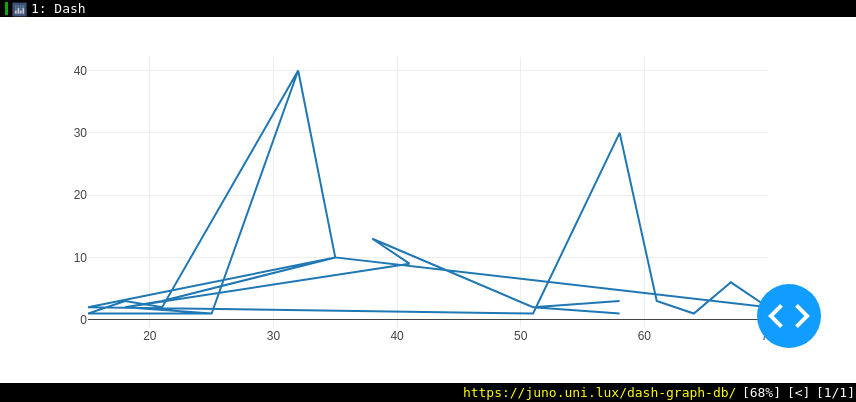
\includegraphics[width=\linewidth]{images/dash-DB-demo.png}
	\caption{\gls{ms} graph relying on \gls{e4l} DB}
	\label{fig:dash-db}
\end{figure*}

\subsubsection{Containerize the application}

Both our solutions---for the API and for the database---were in the
end nothing more than a single Python script. Containerising this was
therefore as simple as copying the files into the container and
execute them using Python. This lead to an unexpected issue however
where the Dash page would not render any graph for both the API and
database solutions.

Extensive experimentation using dummy code and our actual
solutions\footnote{We only experimented on the API version, as the
	database version required us to work on the Juno server and the
	issue was analogous in both solutions. It was simply a matter of
convenience It was simply a matter of convenience.} clearly indicated
that this issue only appeared if we query for data and launch the Dash
application in the same script file. We further made a lot of research
and experiments but we could not find the cause of this issue or how
to solve it. Few resources on Dash with Docker could be found where
the code resembled what we have created, none containing any answers
to our problem.

Finally, the workaround we implemented was to simply put the query of
data and the plotting of the graph using Dash into separate Python
scripts which we would call one after the other. The querying would
write the results to a file, and the Dash graph would read the
information from this file. This effectively solved this mysterious
issue that only appears inside a Docker container.

\subsubsection{Create pipeline to automate deployment}

Before being able to automate the deployment we had to get familiar
with how to do it manually. Deploying the application to Juno was very
straight forward thanks to the fact that we used a Python application
that does not require any compiling or building. Further our
containerized solution also takes care of everything for running the
code. So in the end we only had to create and launch our docker
container which was as simple as running one single command taking
advantage of docker-compose.

As such, the automated pipeline will need to do nothing more than to
execute this exact command. Given how \gls{e4l} used
docker-in-docker\footnote{GitLab runner executes in a docker
container, and we deploy our container using it.} in the pipeline for
hosting the application, we naturally tried to do the same. But here
again we encountered an issue that is still not solved. For some
reason docker related commands gave birth to a Python docker API
exception, thus making the pipeline fail---which was not observed for
\gls{e4l} which used the same approach.

After a lot of vainly research, our workaround was therefore to not
use docker-in-docker, but to have a new GitLab runner that runs
directly on Juno and not inside a container. As such, the commands in
the pipeline will be executed on Juno directly---exactly the same way
we did manually.

\subsubsection{Update the graph information periodically}

The way our solution was built made it such that data was only
retrieved once when launching the container. If new data gets added to
\gls{e4l}, it would not reflect in the graph as no new data will be
fetched. Our solution to periodically grabbing new data fully took
advantage of our previous solution where we split our script in two;
one taking care of querying the data and the other for making the
graph.

We changed the Dash script in a way where it would read data from a
file---produced by the first script---every time the page is loaded.
So if our first script grabs new data and overwrites the file, the
Dash application will read the data again when reloading the page.
This was a very simple change, so now we just need to periodically
call the data query script in order to update the data.

Given that our code runs in a docker container relying on Linux, the
simplest was to implement a system-wide service---but container local
in this case---that would run the query code every once in a while.
Making a systemd timer service seemed like the best idea as most Linux
distributions use systemd. However, the image that we used in our
container seemingly did not ship with any systemd utilities, although
evidence suggested systemd was probably present.

After a bit of research, we ultimately decided to create a cron job
using the \verb|crontab| utility. We set up this job to run our data
query script every hour. This means that the data file will be updated
every hour, regardless of whether new information is actually present
or not. Thus, if we load or reload the Dash page, the new data will be
read from the file.

\subsection{Assessment}

Regarding the gathering of data from \gls{e4l}, one could further
improve this workflow by better highlighting the existence and
features of the back-end as they seem to be somewhat scattered
throughout the application's documentations and are easy to miss.

Also, given that the endpoints were specifically made to be used by
the front-end, it implies that some of the data obtained is not fully
usable for \textit{general} API usage (i.e. the hard coded data in the
front-end). Further, as could be observed in the implementation of the
back-end endpoints, not all available database and service
functionalities were reachable through the API (i.e. no way to
directly query all answers for making statistics). A tight coupling of
front- and back-end can be observed here.

Taking a step back and disregarding all the big technical roadblocks
we encountered when trying to obtain data from \gls{e4l}, when
containerising our application and when trying to create the automated
pipeline using docker-in-docker, it was actually very simple to set up
this specific \gls{ms}. It essentially only consisted in grabbing the
data, making the graph, and updating the data periodically. Seeing
how---in the end---we had a very precise entry point into \gls{e4l}
for obtaining the data, we had a lot of freedome in how to actually
process the data. The isolation of \glspl{ms} therefore provided us
great flexibility which offered us the opportunity to work with tools
we are most comfortable with.

One should keep in mind however, that this is the first and only
\gls{ms} created for \gls{e4l} at this point in time, so we did not
have to worry about managing clusters of services and taking care of
all the complexities that come along with them. We were able to work
with a simplified example of \glspl{ms}.

% \KB{Was is easy to deploy \gls{ms}? Flaws in the service that still
% need to be treated? (i.e. availability of \gls{e4l})}

A few things that are interesting to note now are that our \glspl{ms}
are hosted in a different place from the \gls{e4l} code, which further
accentuates the independence of \glspl{ms}.

Further, the deployment of both our API and database solutions are the
exact same thanks to the docker utilities. Inside these docker
configurations there are slight differences, but they do not reflect
in the actual deployment process. In fact, both deployments are
completely unrelated from each other given that each solution has its
own pipeline and repository. Making changes to one \gls{ms} will not
have an impact on the other one, since there is no common code base
between the two. We only need \gls{e4l} to be running for both
solutions to function.

% \KB{highlight interesting insights: deployment of API \& DB is the
% same. Independent: own repo and pipeline (so no impact on other
% \gls{ms}). Pipeline made it simpler/faster to deploy? Problems
% encountered? What helped to solve them?}

To assess our initial goal of finding out how easy it is to deploy a
\gls{ms}, one has to note that it was quite a bumpy ride all along due
to the many unexpected and inexplicable issues encountered. However,
once we finally had our automated pipeline we did not need to worry
about anything anymore. We simply push our changes to the repository,
and the application will automatically be redeployed without any
further intervention. After going through the manual steps, and
automating them, we have indeed achieved a state where deploying a
\gls{ms} is very simple and fast.
